\section{Roughness propagation}
As described in section \ref{subsec:roughness_prop}, three different test cases
were setup to verify the propagation of the surface roughness values to the
correct volume cells.

\paragraph{Cube}
This test was designed to make sure the propagation is sound. Figure
\ref{fig:cube_ks_prop} shows the surface cube with the rough patch in the middle
of each face. The volume mesh is sliced in two axis and the propagation of the
roughness values can be seen.

\begin{figure}[H] \centering
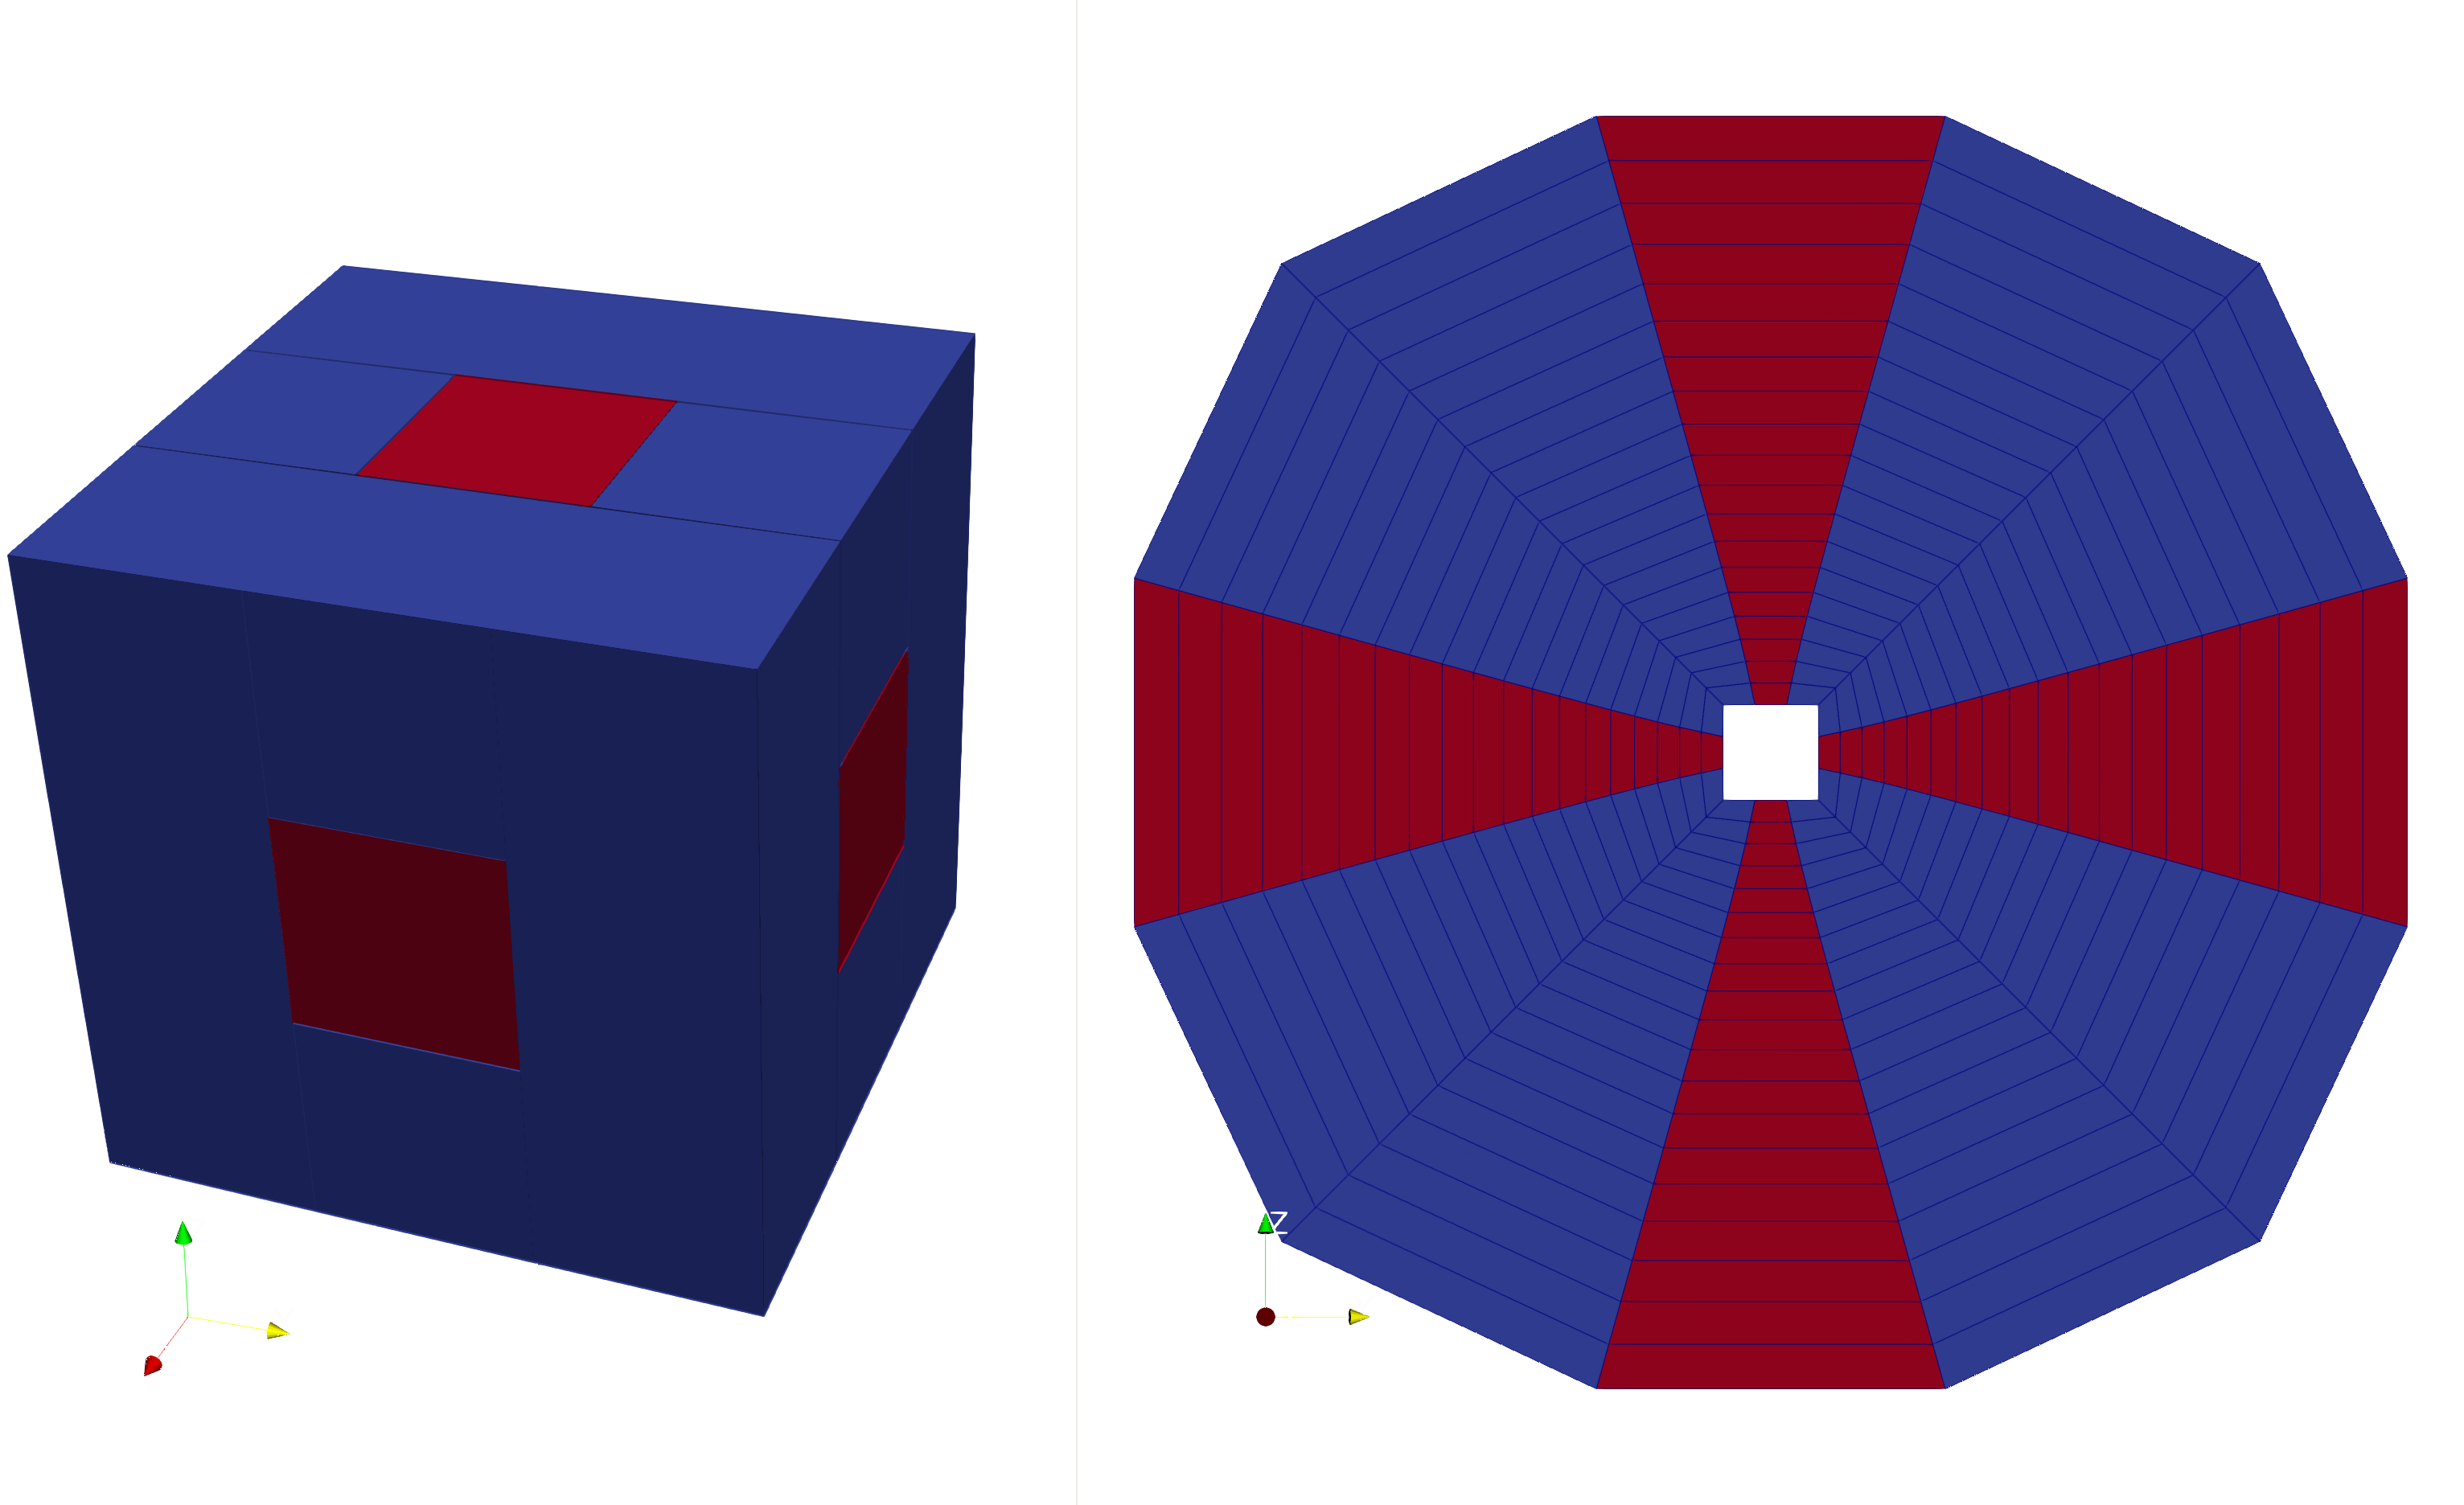
\includegraphics[width=0.7\textwidth]{cube_ks_prop.png}
    \caption{Cube with propagated roughness values. Red equals
$k_{s} = 1.0$ and blue $k_{s} = 0.1$.}
    \label{fig:cube_ks_prop}
\end{figure}

\paragraph{Overset cube}
Similar to the previous test, is used to show that the roughness values are
propagated correctly for  overset meshes. As described in section
\ref{subsec:roughness_prop}, it was necessary to refine the mesh a bit. This was
needed as the \textit{implicit hole cutting} would fail otherwise. In figure
\ref{fig:cube_overset_ks_prop}, the two overlapping meshes with the correctly
propagated roughness values is shown.

\begin{figure}[H] \centering
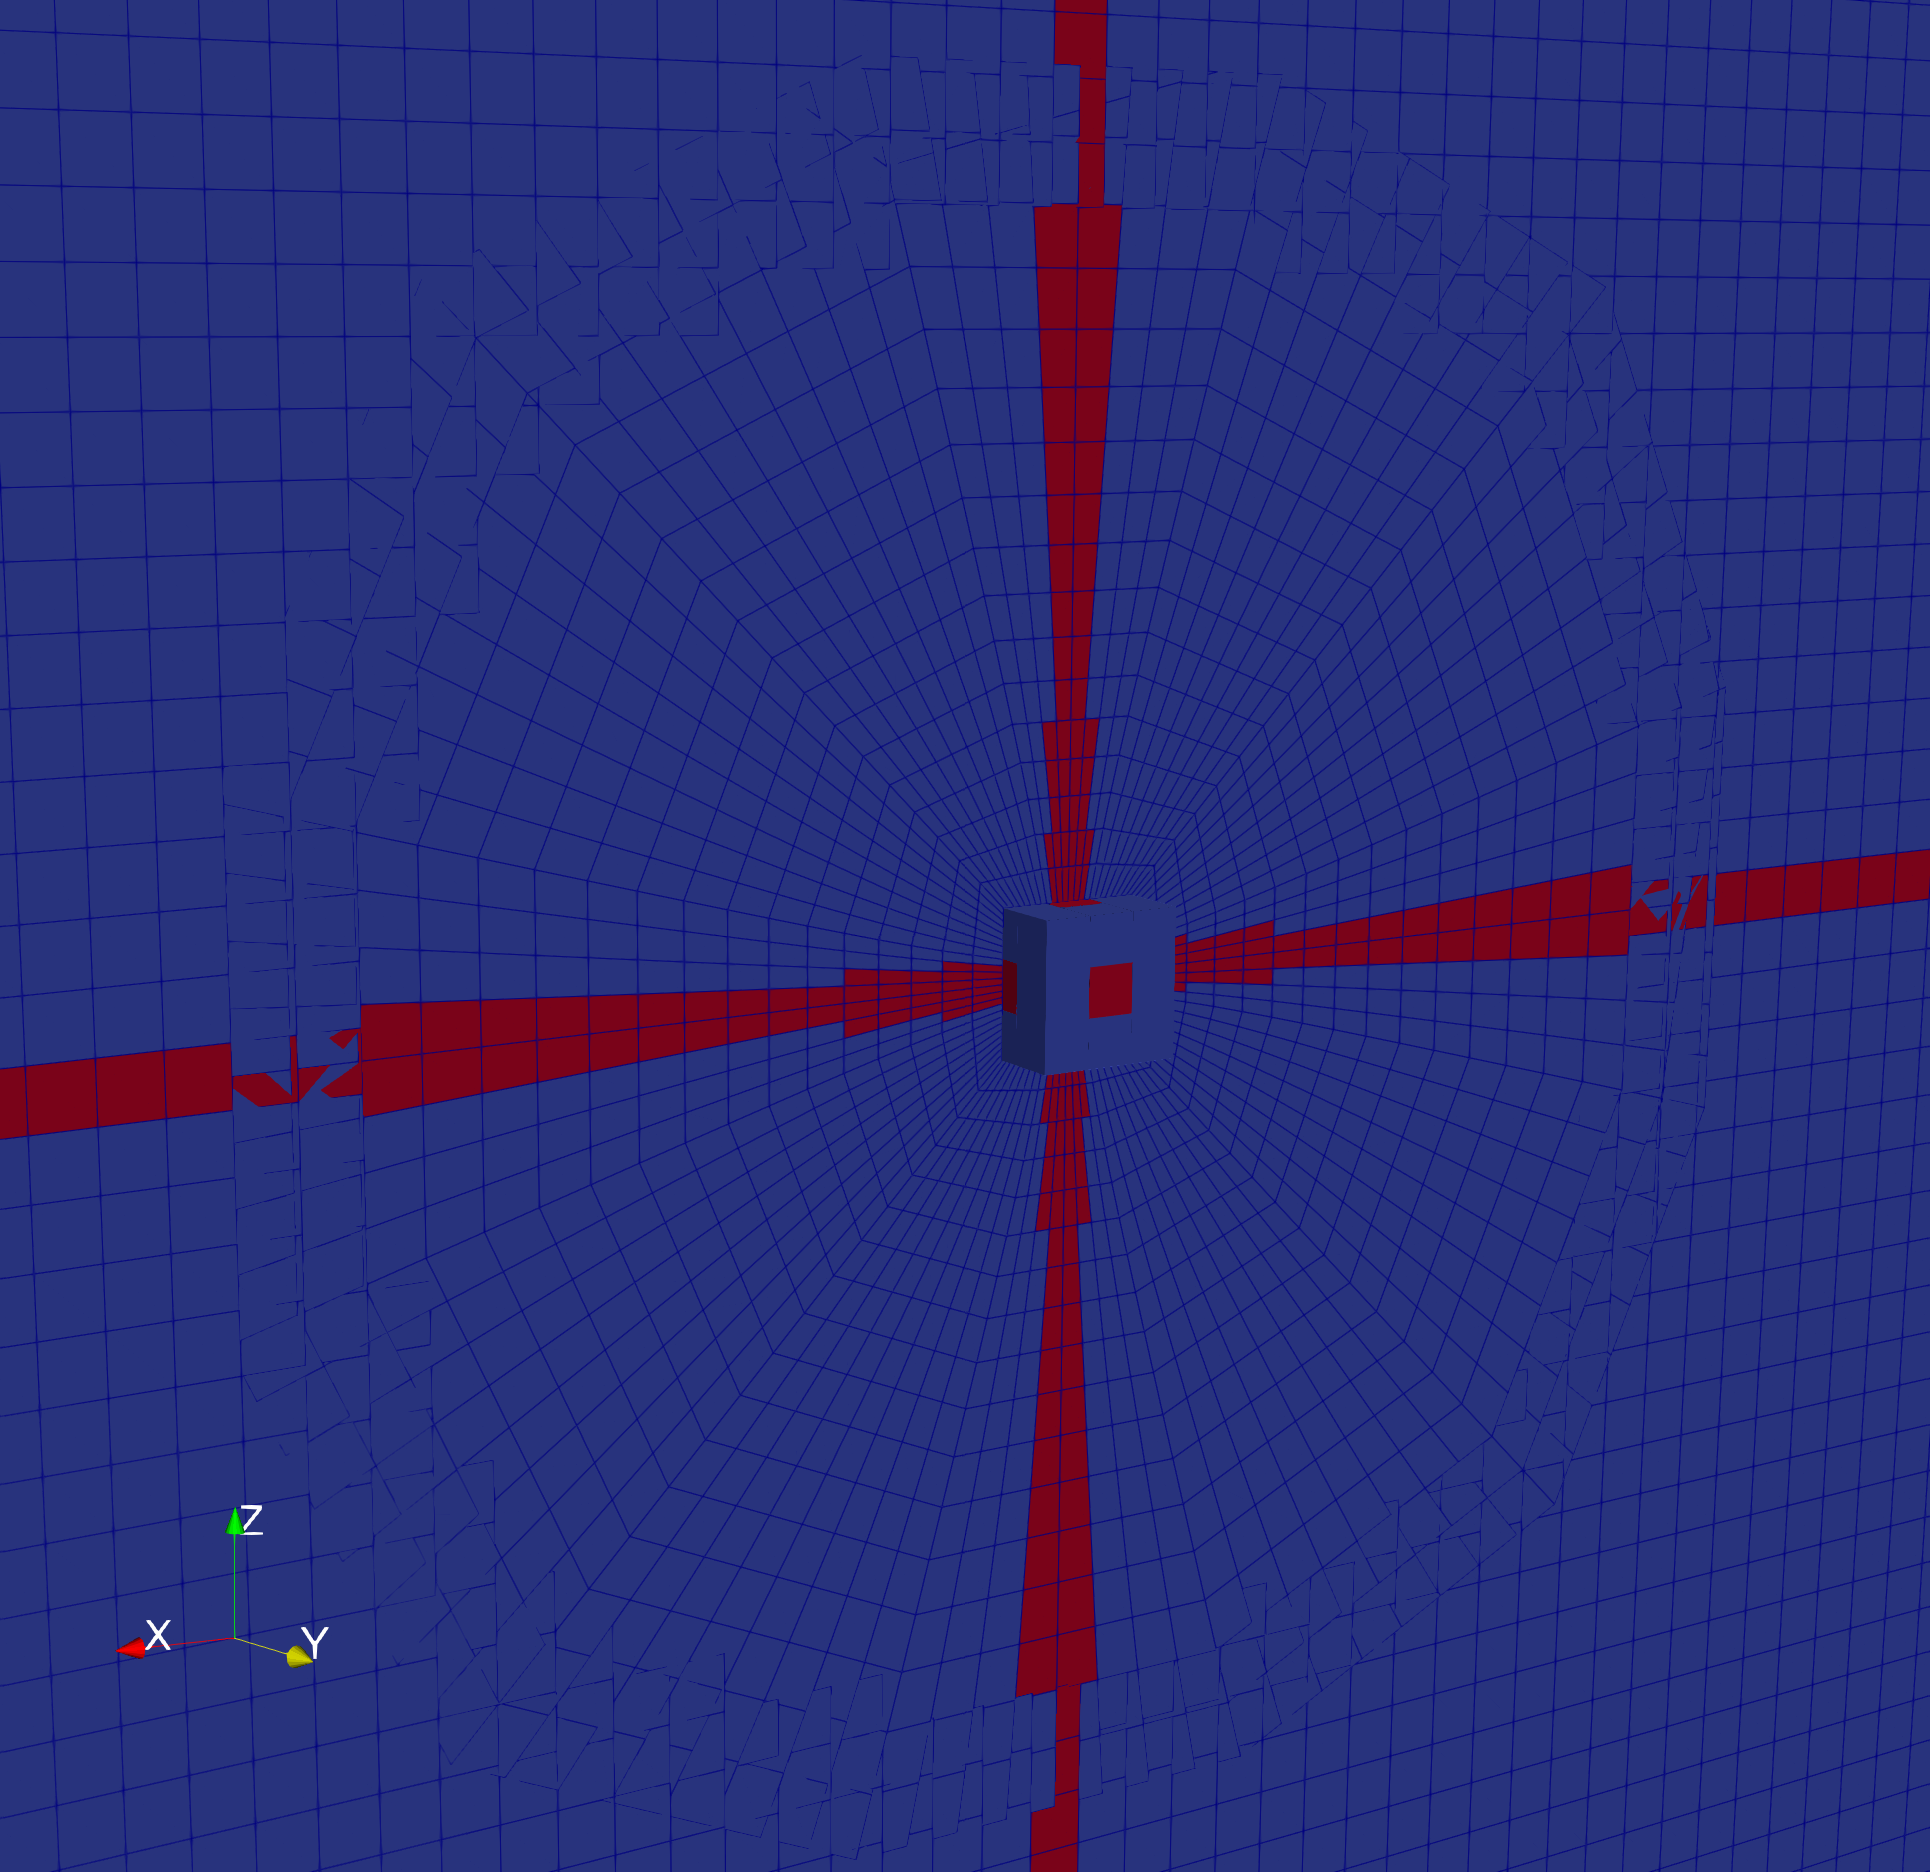
\includegraphics[width=0.7\textwidth]{cube_overset_ks_prop.png}
    \caption{Overset cube with propagated roughness values. Red equals
$k_{s} = 1.0$ and blue $k_{s} = 0.1$.}
    \label{fig:cube_overset_ks_prop}
\end{figure}

\paragraph{Cuboid}
As described in section \ref{subsec:roughness_prop}, this 6 test cases were
designed to catch errors in the correlation of the surface cell to the global
cell index (\texttt{gid}). As such, no figures have been generated. But the
author is happy report that all tests have passed.

\section{Solution comparisons}


\section{Automated tests}
